\documentclass{beamer}

\usepackage[utf8]{inputenc}
\usepackage{minted}

\useoutertheme{infolines}
\beamertemplatenavigationsymbolsempty

\AtBeginSection{\frame{\sectionpage}}
\AtBeginSubsection{\frame{\subsectionpage}}


\title{Introduction to SSH and Ansible}
\author{Guillaume Hélouis}


\begin{document}

\begin{frame}
  \titlepage
\end{frame}

\section{SSH}
\begin{frame}{Overview}
  \begin{itemize}
    \item Identify yourself on SSH servers with SSH keys
    \item No password is ever sent over the network (no bruteforce, MiM
      possibility)
    \item Transparent high security!
    \item Possibility to use a a different key per server
  \end{itemize}
\end{frame}

\begin{frame}{Asymmetric cryptography 101}
  \begin{columns}[T]
    \begin{column}[T]{5cm}
      SSH keys are generated in pairs:
      \begin{itemize}
        \item a private key
        \item a public key
      \end{itemize}
    \end{column}
    \begin{column}[T]{5cm}
      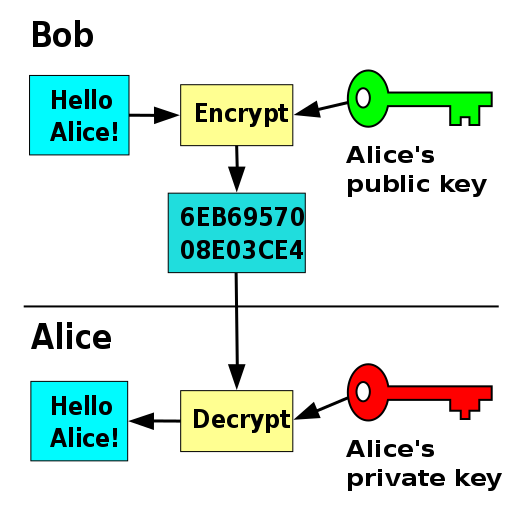
\includegraphics[height=5cm]{images/public_key.png}
    \end{column}
  \end{columns}
\end{frame}

\begin{frame}{Hands-on}
  \begin{itemize}
    \item Check server access: {\tt ssh user@server -p SSH\_PORT}
    \item Generate key pair: {\tt ssh-keygen}
    \item Copy to server: {\tt ssh-copy-id user@server -p SSH\_PORT}
  \end{itemize}
\end{frame}

\begin{frame}{Hands-on}
  \begin{itemize}
    \item Add ssh key to ssh-agent:
      \begin{itemize}
        \item {\tt ssh-agent bash}
        \item {\tt ssh-add \textasciitilde/.ssh/id\_rsa}
      \end{itemize}
  \end{itemize}
\end{frame}

\begin{frame}[fragile]{Config}
  \begin{itemize}
    \item Replace {\tt ssh user@server -p port -i identity-file}
  \end{itemize}
  \begin{exampleblock}{\tt \textasciitilde/.ssh/config} {
      \begin{minted}{shell}
        # global options
        User user

        # host-specific options
        Host myserver
        HostName server-address
        Port port
        IdentityFile ~/.ssh/id_rsa_other
      \end{minted}
    }
  \end{exampleblock}
\end{frame}

\section{Ansible}
\begin{frame}{Intro}
  \begin{center}
    
\includegraphics[height=2cm]{images/ansible_logo.png}
  \end{center}
  \begin{itemize}
    \item Python / free software / supported by Red Hat
    \item Automation: configure servers, deploy stuff\ldots Anything doable
      via CLI
    \item Agent-less
    \item Relies on SSH
    \item Nice learning curve
  \end{itemize}
\end{frame}

\begin{frame}{Why?}
  \begin{center}
    
\includegraphics[height=2.5cm]{images/pet_vs_cattle.jpg}
  \end{center}
  \begin{center}
    Pet vs Cattle
  \end{center}
  \pause
  \begin{itemize}
    \item Immutability % aka immuabilité
  \end{itemize}
\end{frame}

\begin{frame}{Ad-Hoc Commands}
  \begin{itemize}
    \item {\tt ansible -i hosts all -m ping}
    \item {\tt  ansible -i hosts all -a "echo hello"}
  \end{itemize}
\end{frame}

\begin{frame}{Playbooks}
  \begin{itemize}
    \item Ansible scripts in YML
    \item Standard way to organize
    \item Can be version controlled
    \item Community-made playbooks: \href{https://galaxy.ansible.com/search}{Ansible Galaxy}
  \end{itemize}
\end{frame}

\begin{frame}[fragile]{Structure}
  \begin{exampleblock}{} {
      \begin{minted}{text}
        |-- hosts
        |-- playbook.yml
        |-- roles
            |-- my-role
                |-- tasks
                    |-- main.yml
      \end{minted}
    }
  \end{exampleblock}
\end{frame}

\begin{frame}[fragile]{My first playbook}
  \begin{exampleblock}{\tt playbook.yml} {
      \begin{minted}{yaml}
        ---
        - hosts: all
          remote_user: me
          roles:
          - my-role
      \end{minted}
    }
  \end{exampleblock}
\end{frame}

\begin{frame}{Hands-on}
  \begin{itemize}
    \item Clone ansible playbook at \href{https://github.com/ghelouis/agame-player-playbook}{https://github.com/ghelouis/agame-player-playbook}
    \item {Complete missing parts indicated by TODO}
  \end{itemize}
\end{frame}

\begin{frame}{Modules}
  \begin{itemize}
    \item copy
    \item file
  \end{itemize}
\end{frame}

\begin{frame}[fragile]{Answer: Copy jar to HOME}
  \begin{exampleblock}{\tt main.yml} {
      \begin{minted}{yaml}
        - name: copy jar
          copy:
            src: "{{ jar_src }}"
            dest: "{{ ansible_env.HOME }}"
      \end{minted}
    }
  \end{exampleblock}
\end{frame}

\begin{frame}[fragile]{Answer: Remove jar}
  \begin{exampleblock}{\tt main.yml} {
      \begin{minted}{yaml}
      - name: remove jar
        file:
          path: "{{ jar }}"
          state: absent
      \end{minted}
    }
  \end{exampleblock}
\end{frame}

\section{Resources}
\begin{frame}
  \begin{itemize}
    \item \href{https://wiki.archlinux.org/index.php/Secure\_Shell}{wiki.archlinux.org/index.php/Secure\_Shell}
    \item \href{https://wiki.archlinux.org/index.php/SSH\_keys}{wiki.archlinux.org/index.php/SSH\_keys}
    \item \href{https://help.github.com/articles/connecting-to-github-with-ssh/}{help.github.com/articles/connecting-to-github-with-ssh/}
    \item \href{https://en.wikipedia.org/wiki/Public-key\_cryptography}{en.wikipedia.org/wiki/Public-key\_cryptography}
    \item \href{https://docs.ansible.com/}{docs.ansible.com/}
  \end{itemize}
\end{frame}

\end{document}
